\usetheme{ugm1}

% Frame title and footline spacing adjustment
\setbeamertemplate{frametitle}{\vspace*{0.65cm}\hspace*{-0.25cm}%
\begin{beamercolorbox}[wd=0.92\textwidth, ht=0cm, dp=0.35cm]{frametitle}\insertframetitle%
\end{beamercolorbox}}

\setbeamertemplate{footline}{\vspace*{0.60cm}}

\usepackage{booktabs}
\usepackage{array}
\usepackage{amsmath}
\usepackage{graphicx}

% Repository URLs
\newcommand{\repourl}{https://github.com/yusufimantaka/deep-learning-matkul}
\newcommand{\notebookurl}{https://github.com/yusufimantaka/deep-learning-matkul/blob/main/main.ipynb}

% Presentation Metadata
\title{MNIST Classification and\\Regularization Strategies}
\subtitle{{\fontsize{10}{13}\selectfont Yusuf Imantaka Bastari\\[2pt] 24/532731/PA/22530\\[2pt] Magister Kecerdasan Artifisial\\[2pt] Departemen Ilmu Komputer dan Elektronika\\[2pt] FMIPA Universitas Gadjah Mada}}
\author{Yusuf Imantaka Bastari}
\date{\today}

\begin{document}

% =============================================================== Page 1: Identity
\maketitle

% =============================================================== Page 2: URL of Code
{
\usebackgroundtemplate{\backgroundcontent}
\begin{frame}
    \frametitle{Project Repository and Code URL}
    \vspace{0.15cm}
    \begin{block}{GitHub Repository}
        \footnotesize\url{\repourl}
    \end{block}
    
    \vspace{0.15cm}
    \begin{block}{Interactive Jupyter Notebook (main.ipynb)}
        \footnotesize\url{\notebookurl}
    \end{block}
    
    \vspace{0.25cm}
    \textbf{\footnotesize Implementation Overview (Simplified Technical English):}
    \vspace{0.10cm}
    \begin{itemize}\footnotesize
        \setlength\itemsep{3pt}
        \item \textbf{Replication}: Replicated MNIST digit classification from Learning Strategy lecture slides (pages 14--23) using Keras 3 and TensorFlow backend.
        \item \textbf{Baseline Architecture}: Input $28 \times 28 \times 1 \to$ \texttt{Flatten()} $\to$ \texttt{Dense(64, ReLU)} $\to$ \texttt{Dense(10, Softmax)}, trained with Adam optimizer and Categorical Crossentropy for 10 epochs.
        \item \textbf{Controlled Experiments}: Executed 5 regularization scenarios under fixed random seeds ($42$) with automated loss curves, model summaries, and evaluation logging.
    \end{itemize}
\end{frame}
}

% =============================================================== Page 3: Scenario 2(a) L1
{
\usebackgroundtemplate{\backgroundcontent}
\begin{frame}
    \frametitle{Scenario 2(a): L1 Regularization ($\lambda_1 = 10^{-4}$)}
    \vspace{-0.30cm}
    \begin{columns}[T]
        \begin{column}{0.58\textwidth}
            \textbf{\scriptsize Objective \& Mathematical Formulation:}\\[1pt]
            {\scriptsize $\mathcal{L}_{L1}(\theta) = \mathcal{L}_0(\theta) + \lambda_1 \sum_{j} |w_j|$, with $\lambda_1 = 10^{-4}$. Adds a lasso penalty promoting weight sparsity by zeroing inactive weights.}\\[3pt]
            
            \textbf{\scriptsize Model Architecture (\texttt{model.summary()}):}\\[1pt]
            {\scriptsize
            $\bullet$ Layers: \texttt{Flatten(784)} $\to$ \texttt{Dense(64, ReLU, $L_1$)} $\to$ \texttt{Dense(10)}\\
            $\bullet$ Parameters: 50,240 (dense) + 650 (output) = \textbf{50,890} trainable
            }\\[3pt]
            
            \textbf{\scriptsize Performance Evaluation:}\\[1pt]
            {\scriptsize
            \setlength{\tabcolsep}{3pt}
            \renewcommand{\arraystretch}{0.90}
            \begin{tabular}{lccc}
                \toprule
                \textbf{Split} & \textbf{Loss} & \textbf{Accuracy} & \textbf{Baseline Val} \\
                \midrule
                Training & 0.1684 & 97.63\% & 0.0469 / 98.68\% \\
                Validation & \textbf{0.1760} & \textbf{97.13\%} & 0.0928 / 97.18\% \\
                \bottomrule
            \end{tabular}
            \par\vspace{2pt}
            \textbf{STE Insight}: Gap $|\mathcal{L}_{tr} - \mathcal{L}_{val}| = \mathbf{0.0076}$ ($-83.4\%$ vs baseline $0.0458$), effectively preventing overfitting through weight sparsity.\par
            }
        \end{column}
        
        \begin{column}{0.40\textwidth}
            \vspace{-0.35cm}
            \begin{center}
                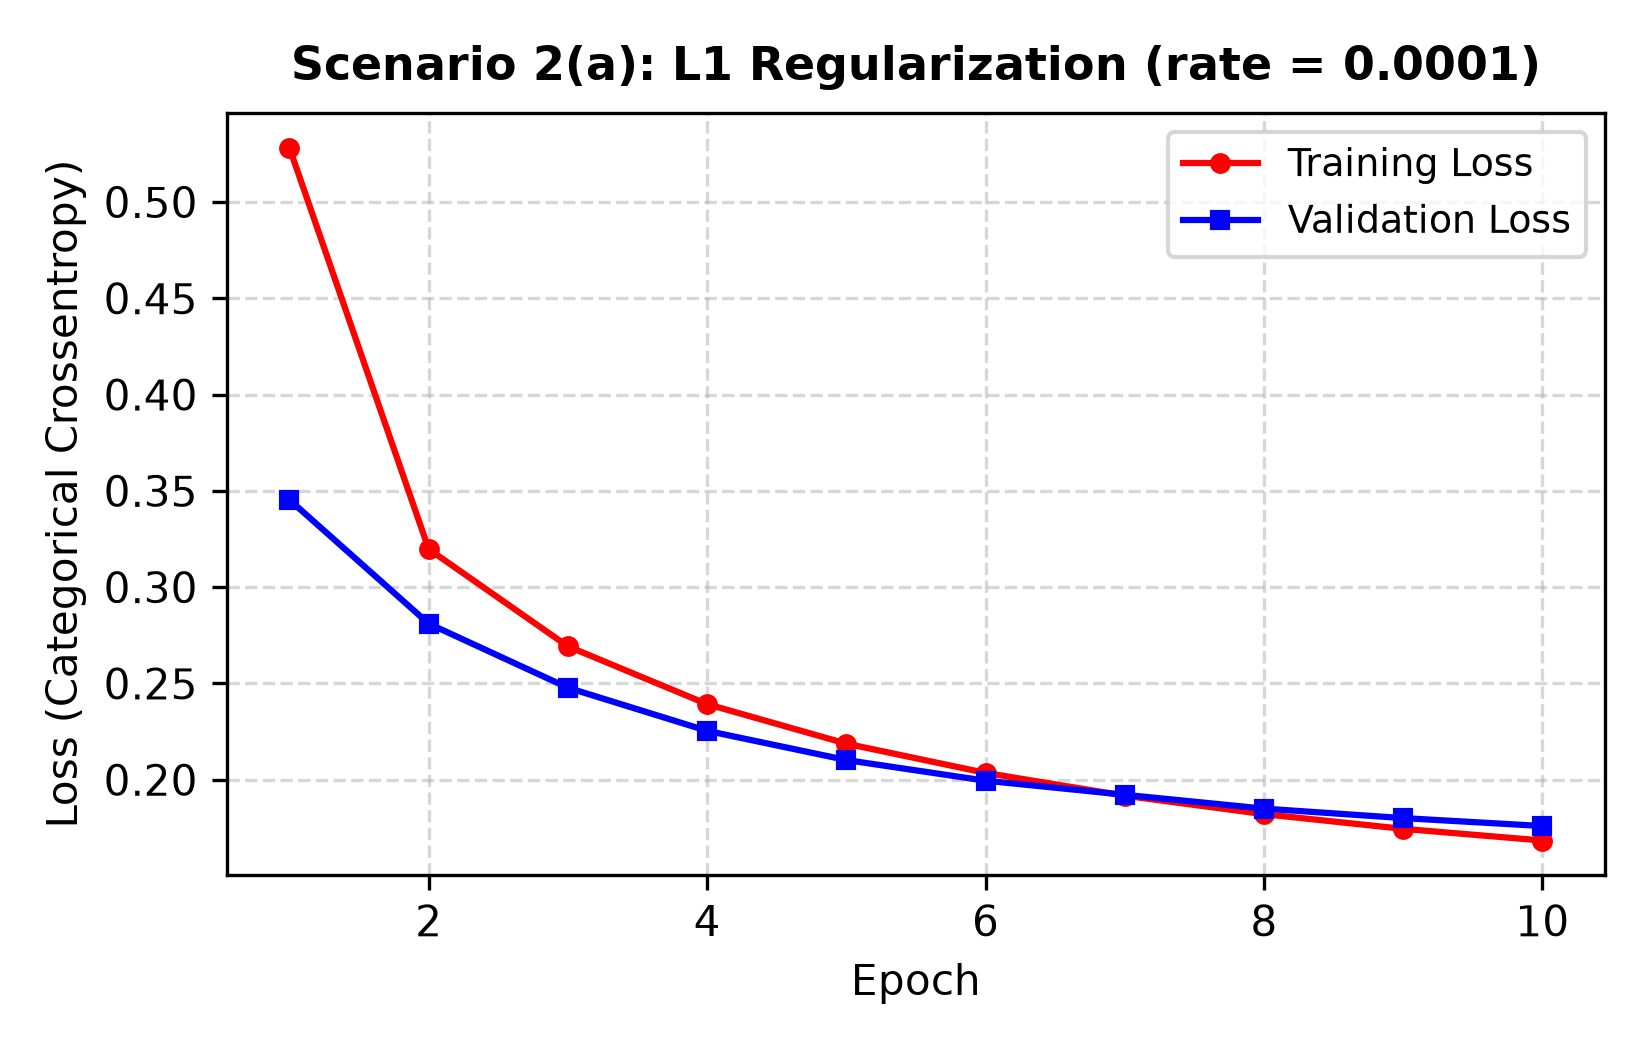
\includegraphics[height=3.3cm, keepaspectratio]{figures/loss_l1.png}
            \end{center}
            \vspace{-8pt}
            {\tiny\centering Figure 1: Training vs. Validation Loss under $L_1$ ($\lambda_1 = 10^{-4}$).\par}
        \end{column}
    \end{columns}
\end{frame}
}

% =============================================================== Page 4: Scenario 2(b) L2
{
\usebackgroundtemplate{\backgroundcontent}
\begin{frame}
    \frametitle{Scenario 2(b): L2 Regularization ($\lambda_2 = 10^{-4}$)}
    \vspace{-0.30cm}
    \begin{columns}[T]
        \begin{column}{0.58\textwidth}
            \textbf{\scriptsize Objective \& Mathematical Formulation:}\\[1pt]
            {\scriptsize $\mathcal{L}_{L2}(\theta) = \mathcal{L}_0(\theta) + \frac{1}{2}\lambda_2 \sum_{j} w_j^2$, with $\lambda_2 = 10^{-4}$. Weight decay penalizes large weights quadratically, bounding parameter norm.}\\[3pt]
            
            \textbf{\scriptsize Model Architecture (\texttt{model.summary()}):}\\[1pt]
            {\scriptsize
            $\bullet$ Layers: \texttt{Flatten(784)} $\to$ \texttt{Dense(64, ReLU, $L_2$)} $\to$ \texttt{Dense(10)}\\
            $\bullet$ Parameters: 50,240 (dense) + 650 (output) = \textbf{50,890} trainable
            }\\[3pt]
            
            \textbf{\scriptsize Performance Evaluation:}\\[1pt]
            {\scriptsize
            \setlength{\tabcolsep}{3pt}
            \renewcommand{\arraystretch}{0.90}
            \begin{tabular}{lccc}
                \toprule
                \textbf{Split} & \textbf{Loss} & \textbf{Accuracy} & \textbf{Baseline Val} \\
                \midrule
                Training & 0.0874 & 98.26\% & 0.0469 / 98.68\% \\
                Validation & \textbf{0.1170} & \textbf{97.19\%} & 0.0928 / 97.18\% \\
                \bottomrule
            \end{tabular}
            \par\vspace{2pt}
            \textbf{STE Insight}: Sustains high test accuracy ($97.19\%$). Quadratic weight decay ensures smooth distribution without sharp zero coefficients.\par
            }
        \end{column}
        
        \begin{column}{0.40\textwidth}
            \vspace{-0.35cm}
            \begin{center}
                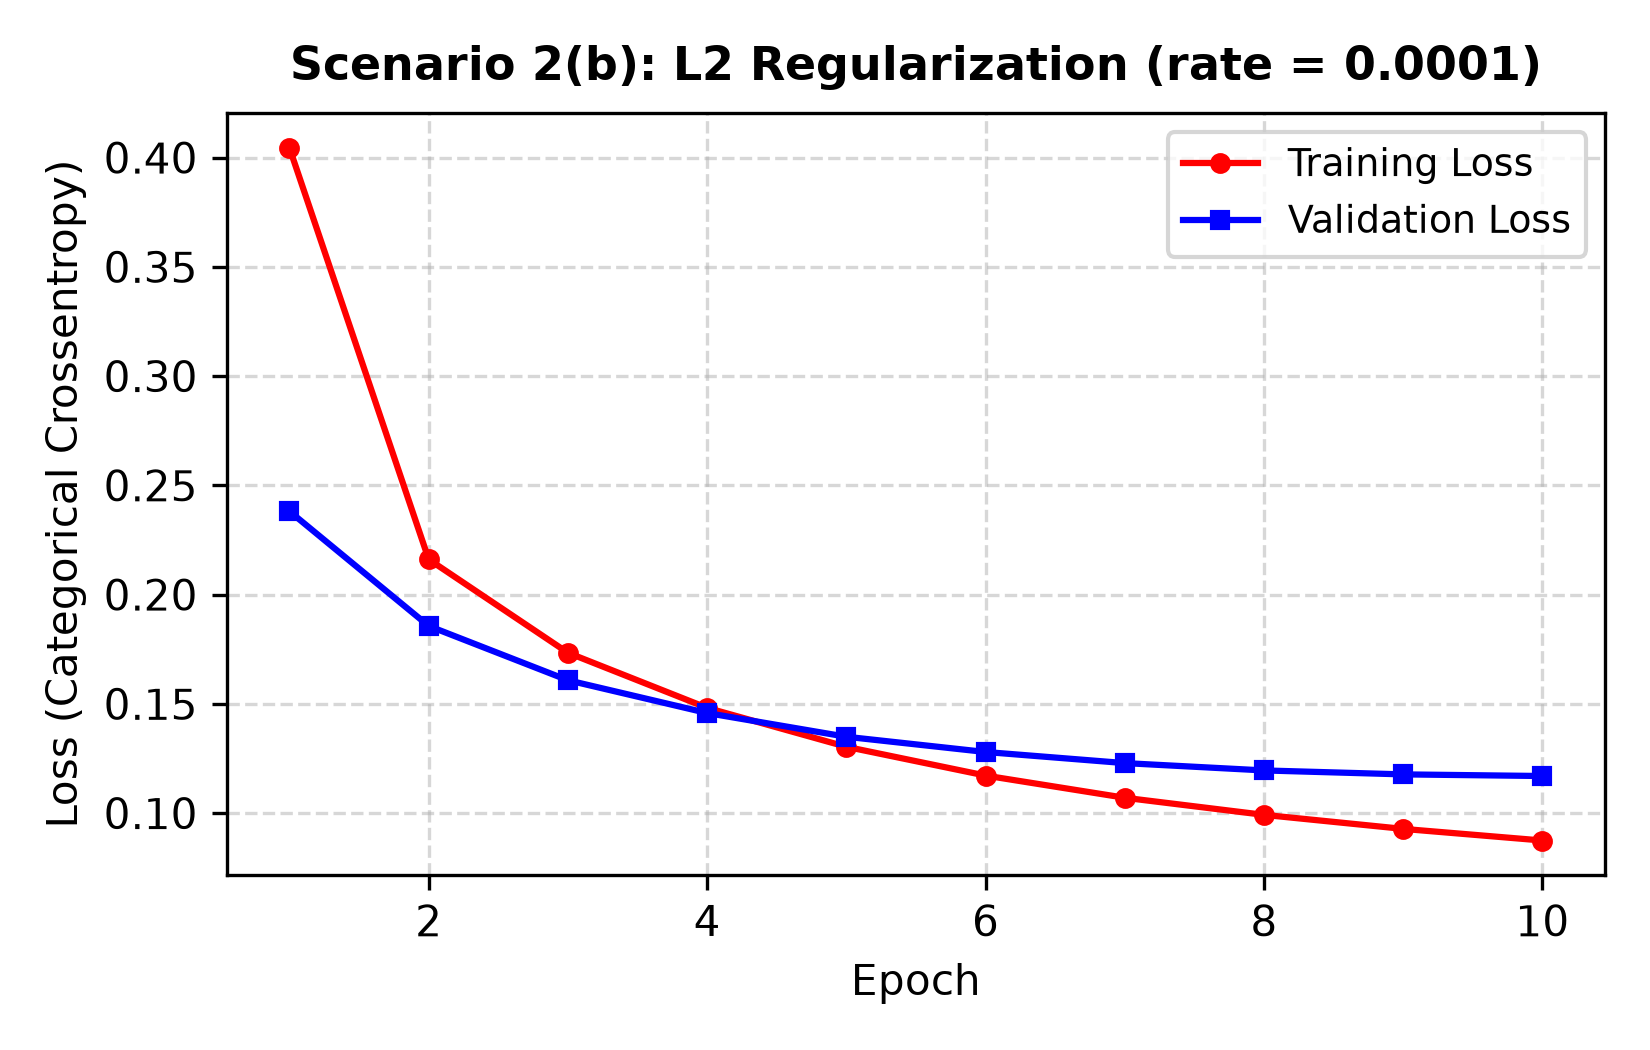
\includegraphics[height=3.3cm, keepaspectratio]{figures/loss_l2.png}
            \end{center}
            \vspace{-8pt}
            {\tiny\centering Figure 2: Training vs. Validation Loss under $L_2$ ($\lambda_2 = 10^{-4}$).\par}
        \end{column}
    \end{columns}
\end{frame}
}

% =============================================================== Page 5: Scenario 2(c) Dropout
{
\usebackgroundtemplate{\backgroundcontent}
\begin{frame}
    \frametitle{Scenario 2(c): Dropout ($p = 0.2$)}
    \vspace{-0.30cm}
    \begin{columns}[T]
        \begin{column}{0.58\textwidth}
            \textbf{\scriptsize Objective \& Mathematical Formulation:}\\[1pt]
            {\scriptsize $\tilde{h} = \frac{1}{1-p}(h \odot r), \ r_j \sim \text{Bernoulli}(1-p)$, with $p = 0.2$. Randomly disables 20\% of hidden units per minibatch to break co-adaptation.}\\[3pt]
            
            \textbf{\scriptsize Model Architecture (\texttt{model.summary()}):}\\[1pt]
            {\scriptsize
            $\bullet$ Layers: \texttt{Flatten(784)} $\to$ \texttt{Dense(64, ReLU)} $\to$ \texttt{Dropout(0.2)} $\to$ \texttt{Dense(10)}\\
            $\bullet$ Parameters: 50,240 (dense) + 650 (output) = \textbf{50,890} trainable
            }\\[3pt]
            
            \textbf{\scriptsize Performance Evaluation:}\\[1pt]
            {\scriptsize
            \setlength{\tabcolsep}{3pt}
            \renewcommand{\arraystretch}{0.90}
            \begin{tabular}{lccc}
                \toprule
                \textbf{Split} & \textbf{Loss} & \textbf{Accuracy} & \textbf{Baseline Val} \\
                \midrule
                Training & 0.0975 & 96.93\% & 0.0469 / 98.68\% \\
                Validation & \textbf{0.0872} & \textbf{97.44\%} & 0.0928 / 97.18\% \\
                \bottomrule
            \end{tabular}
            \par\vspace{2pt}
            \textbf{STE Insight}: \textbf{Top Test Accuracy ($97.44\%$)} and lowest validation loss ($0.0872$). Full sub-network ensemble effect at test inference.\par
            }
        \end{column}
        
        \begin{column}{0.40\textwidth}
            \vspace{-0.35cm}
            \begin{center}
                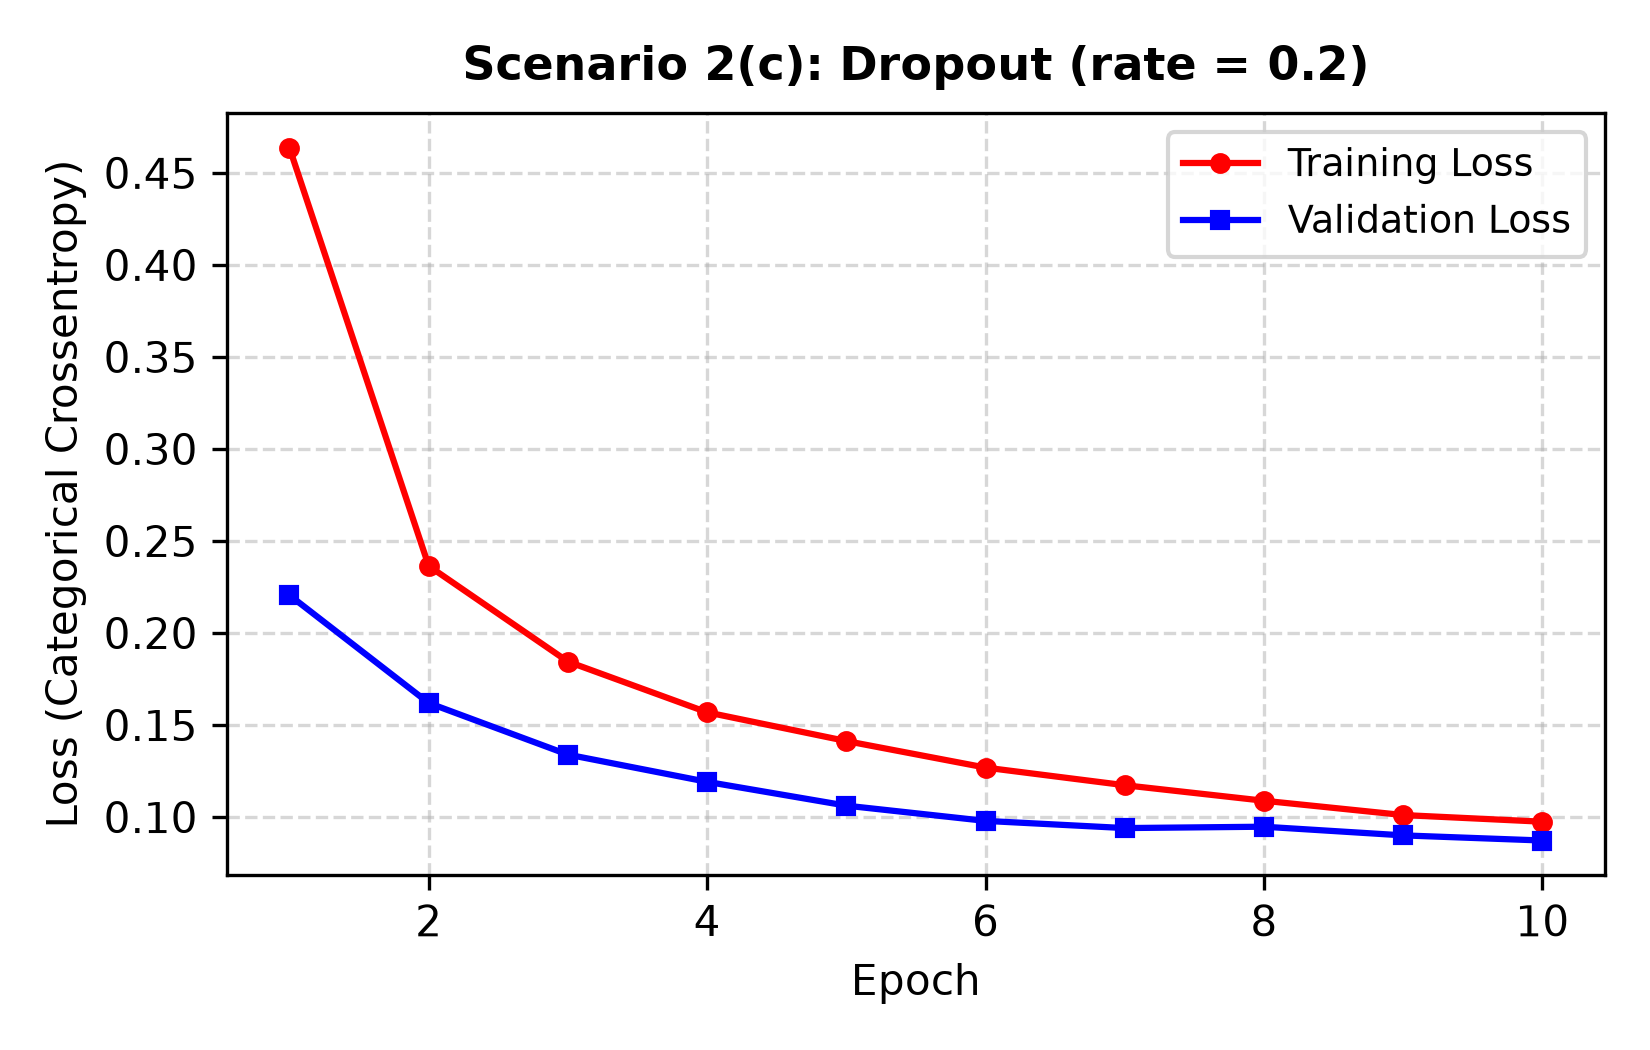
\includegraphics[height=3.3cm, keepaspectratio]{figures/loss_dropout.png}
            \end{center}
            \vspace{-8pt}
            {\tiny\centering Figure 3: Training vs. Validation Loss under Dropout ($p = 0.2$).\par}
        \end{column}
    \end{columns}
\end{frame}
}

% =============================================================== Page 6: Scenario 2(d) Early Stopping
{
\usebackgroundtemplate{\backgroundcontent}
\begin{frame}
    \frametitle{Scenario 2(d): Early Stopping (Patience $k = 3$)}
    \vspace{-0.30cm}
    \begin{columns}[T]
        \begin{column}{0.58\textwidth}
            \textbf{\scriptsize Formulation \& Termination Criteria:}\\[1pt]
            {\scriptsize Monitor $\mathcal{L}_{val}(t)$; halt if $\min_{t' \le t} \mathcal{L}_{val}(t')$ fails to improve for $k=3$ epochs. Restores best weights: $w^* = \arg\min_w \mathcal{L}_{val}(w)$.}\\[3pt]
            
            \textbf{\scriptsize Execution Details \& Model Summary:}\\[1pt]
            {\scriptsize
            $\bullet$ Layers: \texttt{Flatten(784)} $\to$ \texttt{Dense(64, ReLU)} $\to$ \texttt{Dense(10)}\\
            $\bullet$ Terminated: \textbf{Epoch 15} / 25; Restored \textbf{Epoch 12} (Saved 40\% epochs)\\
            $\bullet$ Parameters: \textbf{50,890} trainable (203.55 KB)
            }\\[3pt]
            
            \textbf{\scriptsize Performance Evaluation (at Restored Epoch 12):}\\[1pt]
            {\scriptsize
            \setlength{\tabcolsep}{3pt}
            \renewcommand{\arraystretch}{0.90}
            \begin{tabular}{lccc}
                \toprule
                \textbf{Split} & \textbf{Loss} & \textbf{Accuracy} & \textbf{Baseline Val} \\
                \midrule
                Training (ep 12) & 0.0402 & 98.90\% & 0.0469 / 98.68\% \\
                Validation & \textbf{0.0921} & \textbf{97.16\%} & 0.0928 / 97.18\% \\
                \bottomrule
            \end{tabular}
            \par\vspace{2pt}
            \textbf{STE Insight}: Halts before validation loss diverges, successfully restoring peak parameters while eliminating redundant training cycles.\par
            }
        \end{column}
        
        \begin{column}{0.40\textwidth}
            \vspace{-0.35cm}
            \begin{center}
                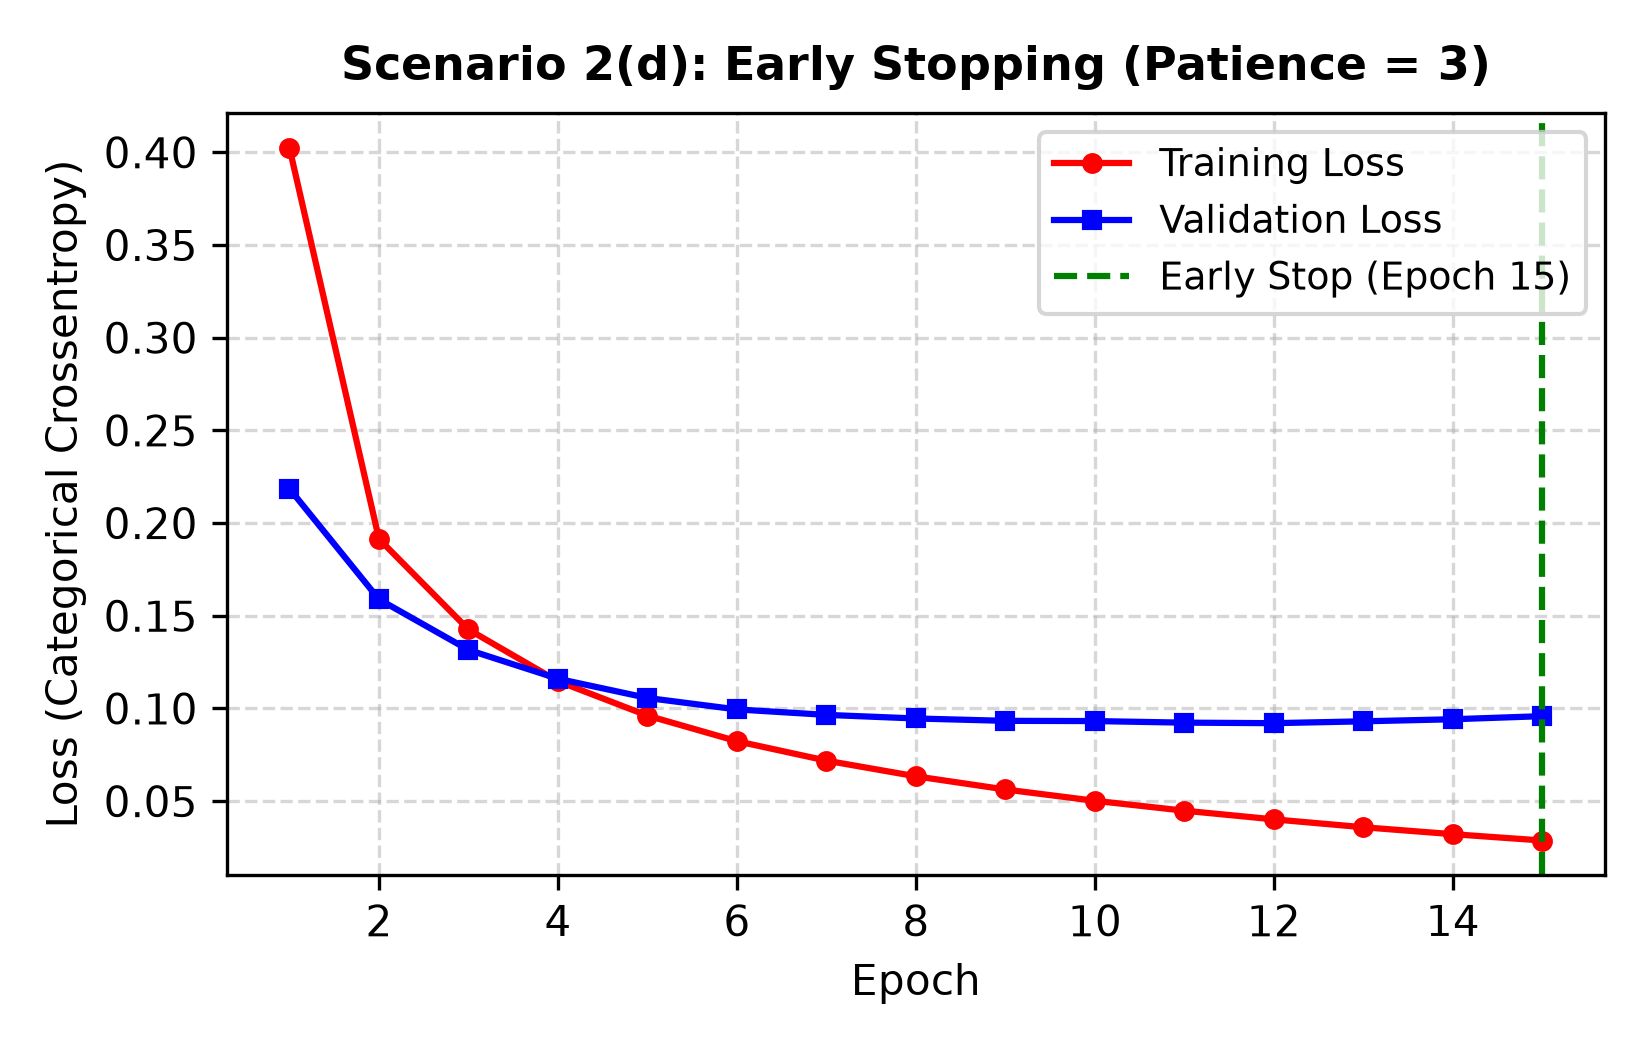
\includegraphics[height=3.3cm, keepaspectratio]{figures/loss_early_stopping.png}
            \end{center}
            \vspace{-8pt}
            {\tiny\centering Figure 4: Training vs. Validation Loss curve. Stopped at ep 15; restored ep 12.\par}
        \end{column}
    \end{columns}
\end{frame}
}

% =============================================================== Page 7: Scenario 2(e) L1 + Dropout
{
\usebackgroundtemplate{\backgroundcontent}
\begin{frame}
    \frametitle{Scenario 2(e): L1 Regularization + Dropout}
    \vspace{-0.30cm}
    \begin{columns}[T]
        \begin{column}{0.58\textwidth}
            \textbf{\scriptsize Compound Regularization Formulation:}\\[1pt]
            {\scriptsize $\mathcal{L}(\theta) = \mathcal{L}_0(\theta) + \lambda_1 \sum |w_j|$ with $\tilde{h} = \frac{1}{1-p}(h \odot r)$. Combines weight sparsity ($\lambda_1 = 10^{-4}$) with neuron de-correlation ($p = 0.2$).}\\[3pt]
            
            \textbf{\scriptsize Model Architecture (\texttt{model.summary()}):}\\[1pt]
            {\scriptsize
            $\bullet$ Layers: \texttt{Flatten(784)} $\to$ \texttt{Dense(64, ReLU, $L_1$)} $\to$ \texttt{Dropout(0.2)} $\to$ \texttt{Dense(10)}\\
            $\bullet$ Parameters: 50,240 (dense) + 650 (output) = \textbf{50,890} trainable
            }\\[3pt]
            
            \textbf{\scriptsize Performance Evaluation:}\\[1pt]
            {\scriptsize
            \setlength{\tabcolsep}{3pt}
            \renewcommand{\arraystretch}{0.90}
            \begin{tabular}{lccc}
                \toprule
                \textbf{Split} & \textbf{Loss} & \textbf{Accuracy} & \textbf{Baseline Val} \\
                \midrule
                Training & 0.2231 & 96.14\% & 0.0469 / 98.68\% \\
                Validation & \textbf{0.1870} & \textbf{97.11\%} & 0.0928 / 97.18\% \\
                \bottomrule
            \end{tabular}
            \par\vspace{2pt}
            \textbf{STE Insight}: Dual constraints prevent over-reliance on individual features. Strong regularizer prevents memorization, producing stable tracking.\par
            }
        \end{column}
        
        \begin{column}{0.40\textwidth}
            \vspace{-0.35cm}
            \begin{center}
                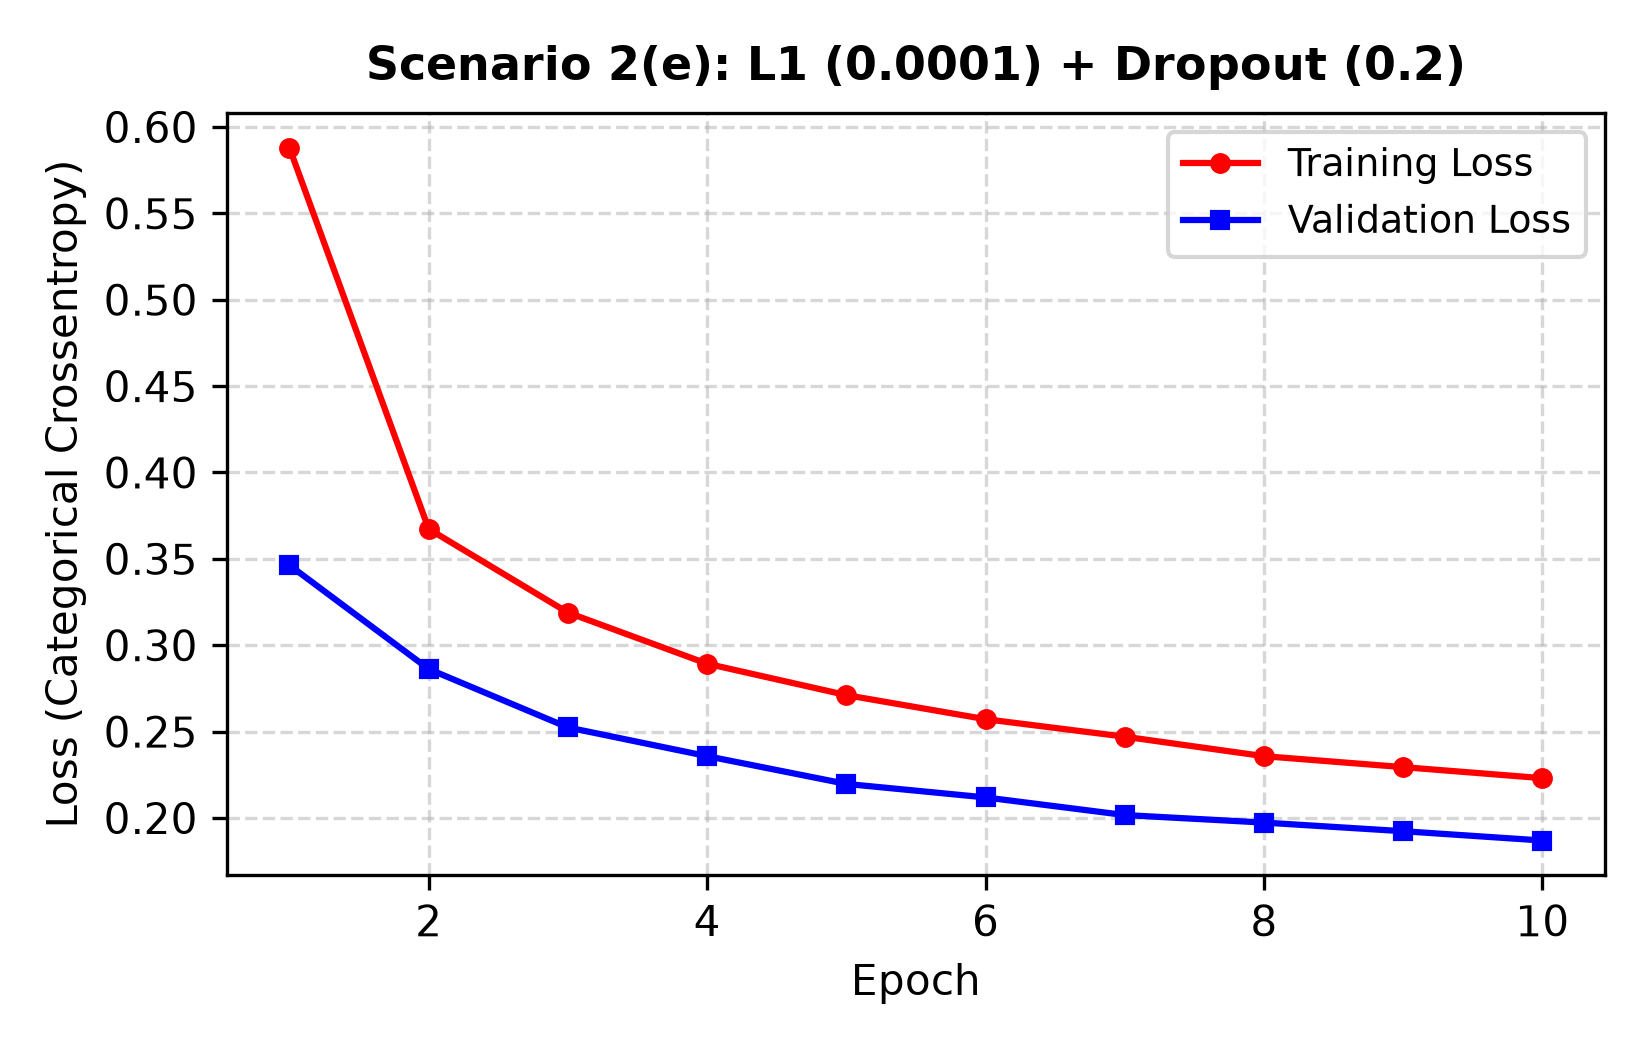
\includegraphics[height=3.3cm, keepaspectratio]{figures/loss_l1_dropout.png}
            \end{center}
            \vspace{-8pt}
            {\tiny\centering Figure 5: Training vs. Validation Loss under joint $L_1$ and Dropout.\par}
        \end{column}
    \end{columns}
\end{frame}
}

% =============================================================== Page 8: Conclusion
{
\usebackgroundtemplate{\backgroundcontent}
\begin{frame}
    \frametitle{Conclusion: Quantitative Synthesis}
    \vspace{-0.20cm}
    \begin{table}[h]
        \centering\scriptsize
        \renewcommand{\arraystretch}{0.92}
        \setlength{\tabcolsep}{4pt}
        \begin{tabular}{lccccc}
            \toprule
            \textbf{Strategy} & \textbf{Hyperparameter} & \textbf{Train Acc} & \textbf{Test Acc} & \textbf{Test Loss} & \textbf{$|\Delta \text{Loss}|$} \\
            \midrule
            Baseline MLP & None & 98.68\% & 97.18\% & 0.0928 & 0.0458 \\
            Scenario 2(a) & $L_1$ ($\lambda_1 = 10^{-4}$) & 97.63\% & 97.13\% & 0.1760 & \textbf{0.0076} \\
            Scenario 2(b) & $L_2$ ($\lambda_2 = 10^{-4}$) & 98.26\% & 97.19\% & 0.1170 & 0.0295 \\
            Scenario 2(c) & Dropout ($p = 0.2$) & 96.93\% & \textbf{97.44\%} & \textbf{0.0872} & 0.0102 \\
            Scenario 2(d) & Early Stopping ($k=3$) & 98.90\% & 97.16\% & 0.0921 & 0.0519 \\
            Scenario 2(e) & $L_1$ ($10^{-4}$) + Dropout ($0.2$) & 96.14\% & 97.11\% & 0.1870 & 0.0361 \\
            \bottomrule
        \end{tabular}
    \end{table}

    \vspace{-0.15cm}
    \textbf{\scriptsize Key Findings (Simplified Technical English):}
    \vspace{0.02cm}
    \begin{itemize}\scriptsize
        \setlength\itemsep{1pt}
        \item \textbf{Generalization Champion}: \textbf{Dropout ($p=0.2$)} produced the highest test accuracy ($97.44\%$) and lowest test loss ($0.0872$) by mitigating hidden neuron co-adaptation.
        \item \textbf{Overfitting Elimination}: \textbf{$L_1$ Regularization} achieved the tightest generalization gap ($0.0076$), reducing loss divergence by $83.4\%$ through weight sparsity.
        \item \textbf{Smooth Weight Bounding}: \textbf{$L_2$ Regularization} prevented dominant weight magnitudes, preserving competitive test accuracy ($97.19\%$).
        \item \textbf{Computational Conservation}: \textbf{Early Stopping} halted at epoch 15 and restored epoch 12 weights, saving $40\%$ of training computation without sacrificing accuracy.
        \item \textbf{Dual Synergy}: Combining $L_1$ and Dropout delivered balanced parameter sparsity and architecture de-correlation.
    \end{itemize}
\end{frame}
}

\end{document}
